\documentclass[a4paper,headlines=4, footlines=1]{scrartcl}
\usepackage{amsmath,amssymb,amsthm,booktabs,braket,graphicx,hyphenat,lmodern,marginnote,microtype,scrpage2,tikz,tikz-3dplot}
\usepackage[utf8]{inputenc}
\let\marginpar\marginnote{}\usepackage[ngerman]{babel}\usepackage[german=quotes]{csquotes}\usepackage[T1]{fontenc}\usepackage{hyperref}\hypersetup{colorlinks=true,linkcolor=black,citecolor=black,filecolor=black,urlcolor=black}\newcommand{\E}{\mathrm{e}}\newcommand{\I}{\mathrm{i}}\newcommand{\de}{\mathrm{d}}\newcommand{\td}[2]{\frac{\de{#1}}{\de{#2}}}\pagestyle{scrheadings} \clearscrheadings\renewcommand{\headfont}{\normalfont}
%\lehead{\pagemark}
%\cehead{}
%\rehead{\headmark}
%\lohead{\rightmark}
%\cohead{}
%\rohead{\pagemark}
\setheadsepline{0.4pt}\setfootsepline{0.4pt}
\usepackage[inner=20mm,marginparsep=5mm,marginparwidth=30mm,outer=30mm,top=30mm,bottom=30mm,footskip=10mm]{geometry}
\usepackage[format=plain,margin=3em,font=small,labelfont=bf,labelsep=endash]{caption}
\renewcommand*{\marginfont}{\footnotesize} %\renewcommand{\vec}{\mathbf}
%\usepackage{kpfonts}
\usetikzlibrary{angles,quotes}
\usepackage{extarrows}
\newcommand{\ray}[1]{\stackrel{\rightharpoonup}{#1}}
\usepackage{tabularx}
\usepackage{tkz-fct}
\usepackage{multirow}
\usepackage{enumerate}
\addto\captionsngerman{%	
	\renewcommand{\figurename}{Abb.}	
	\renewcommand{\tablename}{Tab.}	
}

\ihead{Eberhard Karls Universität Tübingen\\
	Mathematisch-Naturwissenschaftliche Fakultät\\
	Fachdidaktik II: Geometrie\\
	Prof. Dr. Hermann Hähl}
\chead{}
\ohead{\parbox[l]{2.5cm}{A. Bucher\\
		P. Gepperth\\
		S. Jung\\
		J. Stigler}}

\ifoot{Sitzung 2: Zentrische Streckungen}
\cfoot{}
\ofoot{\pagemark}


\title{Handout}

\subtitle{Strahlensätze}

\author{Pascal Gepperth}

\date{\today}

\hypersetup{
    pdftitle={Handout Fachdidaktik Mathematik Strahlensätze},
    pdfauthor={Pascal Gepperth},
	pdfstartview={FitH},
    pdfcreator={LaTeX with TikZ}
}



\begin{document}

\section{Fachwissenschaftliche Auffassung}
\subsection*{Zentrische Streckung}
\subsubsection*{Definition}
Sei $Z$ ein Punkt der Ebene und $k$ eine von Null verschiedene reelle Zahl. Eine Abbildung der Ebene heißt \textit{zentrische Streckung} mit Zentrum $Z$ und Streckfaktor $k$ ($S(Z;k)$), wenn für jeden Punkt $P$ der Ebene gilt:\\\\
(1) Zentrum $Z$, Urbild $P$ und Bild $P'$ liegen auf einer Geraden.\\
(2) Es gilt $ \stackrel{\longrightarrow}{ZP'}=k\stackrel{\longrightarrow}{ZP}$.\\\\\\
Der Faktor $k$ bestimmt den Typ der Abbildung in folgender Weise:\\\\
(1) Ist $k>0$, so liegen Punkt und Bildpunkt auf der selben Seite von $Z$.\\
(2) Ist $k<0$, so liegen Punkt und Bildpunkt auf verschiedenen Seiten von $Z$.\\
(3) Für $k=1$ erhält man die Identität, für $k=-1$ die Punktspiegelung an $Z$.\\
(4) $S(Z;\frac{1}{k})$ ist die Umkehrabbildung von $S(Z;k$).

\subsubsection*{Eigenschaften einer zentrischen Streckung:}
\begin{itemize}
	\item $S(Z;k)$ ist geradentreu. Außerdem sind eine Gerade $g$ und ihre Bildgerade $g'$ stets parallel.
	\item $S(Z;k)$ ist winkeltreu.
	\item Die Bildstrecke einer beliebigen Strecke hat die $|k|$-fache Länge.
	\item $S(Z;k)$ ist verhältnistreu.
\end{itemize}
\subsection*{Verkettungen von zentrischen Streckungen}
Eine zentrische Streckung bildet Geraden parallel ab. Mit dieser Eigenschaft muss auch die Verkettung von zentrischen Streckungen parallel abbilden, und ist somit insbesondere geraden- und parallelentreu. Winkeltreue und Verhältnistreue ergeben sich mit Folgendem:
\\\\ Seien $S(Z_1,k_1),S(Z_2,k_2),\ Z_1\ne Z_2$ zwei zentrische Streckungen, dann gilt: \begin{itemize}
	\item $k_1k_2=1 \Rightarrow S(Z_2,k_2)\circ S(Z_1,k_1)$ ist Verschiebung
	\item $k_1k_2\ne 1 \Rightarrow S(Z_2,k_2)\circ S(Z_1,k_1)$ ist zentrische Streckung mit Zentrum Z Streckfaktor $k=k_1k_2$. 
\end{itemize} 
(Bemerkung: Verschiebungen haben alle Eigenschaften der zentrischen Streckung, sind darüber hinaus sogar längentreu)\\
\begin{figure}[!h]
	\centering
	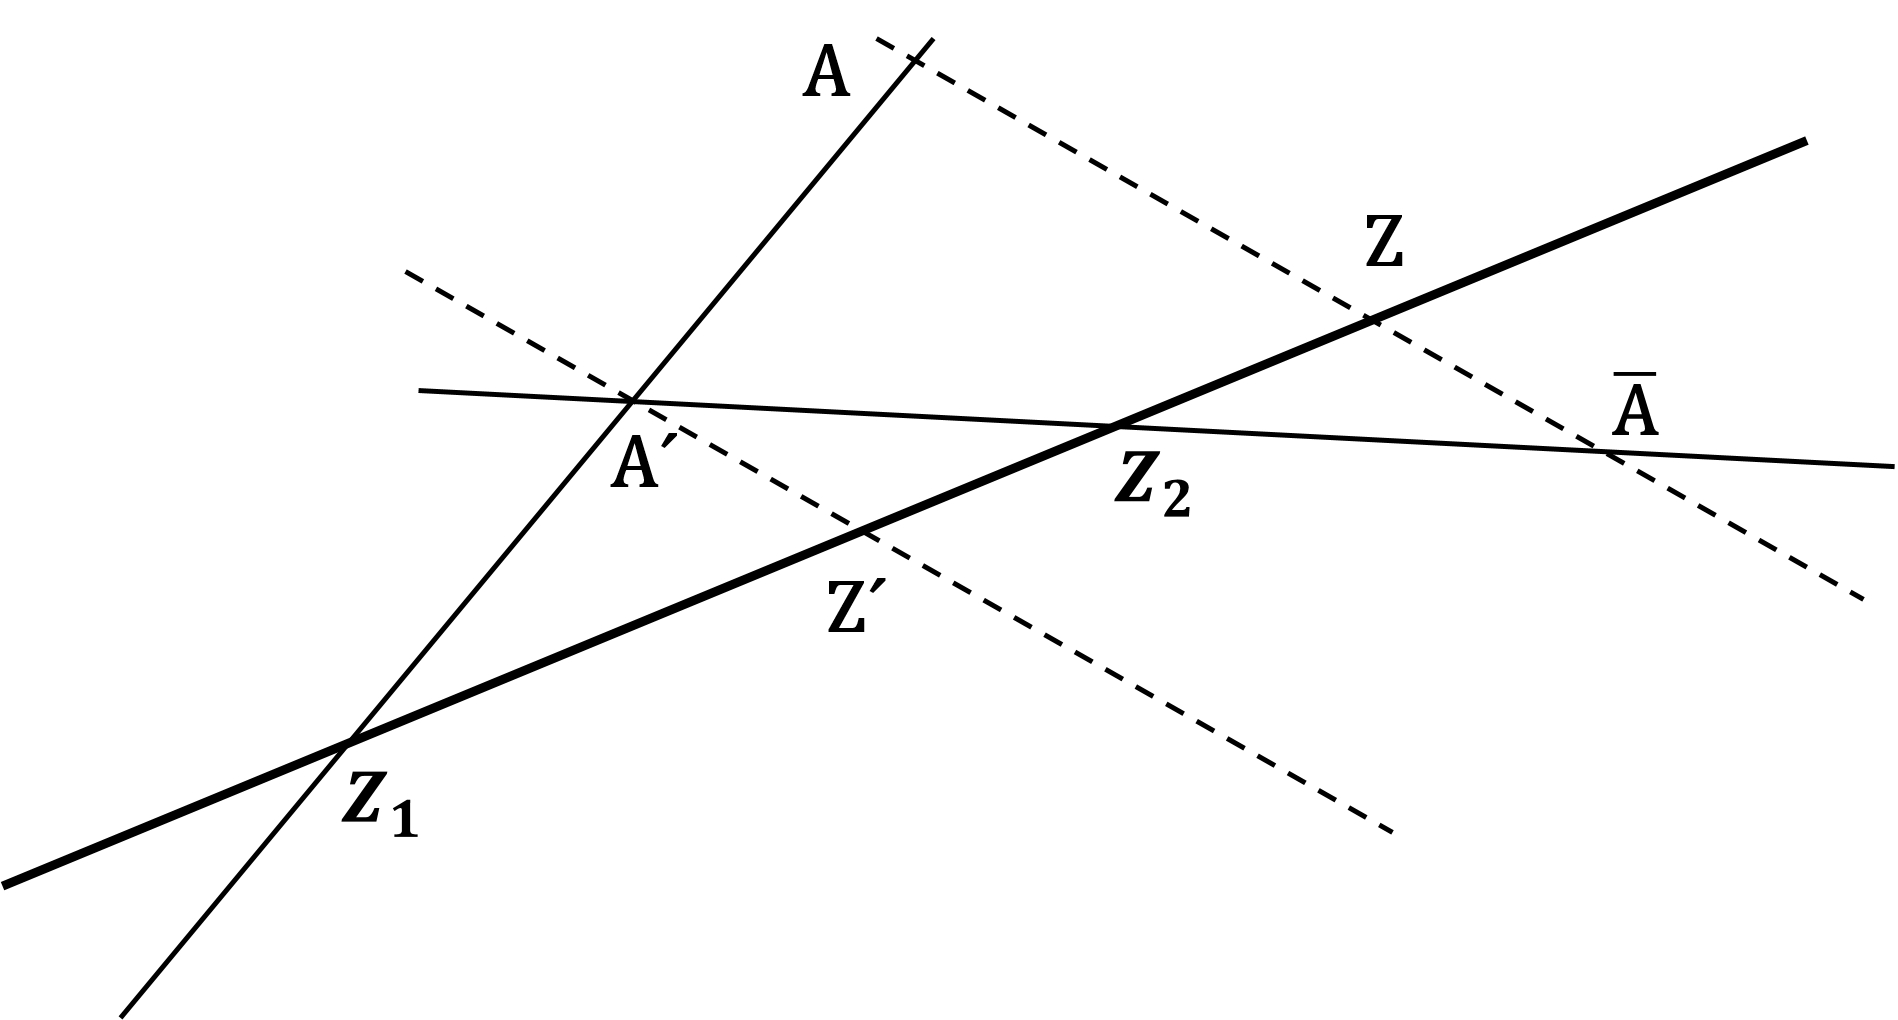
\includegraphics[scale=0.2]{skizzehandout}
\end{figure}\\
Beispiel für Verkettung von zentrischen Streckungen wobei $A\xlongrightarrow{S(Z_1,k_1)}A'\xlongrightarrow{S(Z_2,k_2)}\bar{A}$ und hier $k_1=\frac{1}{2},\ k_2=-1$
\section{Schulische Auffassung}
\paragraph{Definition}
Eine \textbf{zentrische Streckung} wird festgelegt durch das \textbf{Streckzentrum \textit{Z}} und den \textit{positiven} \textbf{Streckfaktor \textit{k}}.\\
Zu einem Punkt erhältst du den Bildpunkt wie folgt:
\begin{enumerate}[(1)]
	\item Wenn der Punkt $ P $ nicht mit dem Zentrum zusammenfällt, dann erhält man den Bildpunkt $ P' $ wie folgt:
	\begin{enumerate}[(a)]
		\item Zeichne die Halbgerade $ \ray{ZP} $.
		\item Zeichne den Punkt $ P' $ auf der Halbgeraden $ \ray{ZP} $ so, dass gilt
		\begin{align*}
		\left|ZP'\right| = k \cdot \left|ZP\right|
		\end{align*}
	\end{enumerate}
	\item Der Bildpunkt $ Z' $ von $ Z $ fällt mit $ Z $ zusammen: $ Z' = Z $.
\end{enumerate}
\paragraph{Zentrische Streckung mit negativem Streckfaktor}
Eingeführt als zentrische Streckung um $ \left|k\right| $ und anschließender Punktspiegelung in $ Z $.
\paragraph{Satz}
Für jede \textit{zentrische Streckung} mit einem positiven Streckfaktor $ k $ gilt:
\begin{enumerate}[(a)]
	\item Gerade und Bildgerade sind parallel.
	\item Bildstrecke ist k-mal so lang wie Originalstrecke.
	\item Winkel und Bildwinkel sind gleich groß.
\end{enumerate}
\end{document}
